% fig_channel_standalone.tex — the released end-to-end channel (fig:channel)
% Build: tectonic fig_channel_standalone.tex   (run from tools/; assets in fig_channel_assets/)
% Style: serif (STIX Two), black/gray line work, single muted blue accent — matches fig_system.
\documentclass[border=6pt]{standalone}
\usepackage{stix2}
\usepackage[T1]{fontenc}
\usepackage{graphicx}
\usepackage{tikz}
\usetikzlibrary{arrows.meta, positioning, calc}
\graphicspath{{fig_channel_assets/}}

\definecolor{accent}{RGB}{60,126,193}% desaturated blue

\begin{document}
\begin{tikzpicture}[
  every node/.style={font=\small},
  box/.style={draw=black, line width=0.7pt, rounded corners=1.5pt, fill=white,
              inner sep=5pt, align=center},
  innerbox/.style={draw=black!80, line width=0.6pt, rounded corners=1pt, fill=white,
                   inner sep=4.5pt, align=center, font=\small},
  group/.style={draw=black, line width=0.8pt, rounded corners=1.5pt, fill=gray!8},
  tier/.style={draw=black!80, line width=0.6pt, rounded corners=1pt, fill=white,
               inner sep=3.5pt, align=center, font=\footnotesize},
  decision/.style={draw=black!80, densely dashed, line width=0.6pt, rounded corners=1.5pt,
                   fill=white, inner sep=4.5pt, align=center, font=\small},
  thumb/.style={draw=black!70, line width=0.5pt, inner sep=0pt},
  flow/.style={-{Stealth[length=2.6mm, width=1.9mm]}, line width=0.8pt},
  loop/.style={-{Stealth[length=2.2mm, width=1.6mm]}, line width=0.7pt, accent},
  gtitle/.style={font=\normalsize\scshape},
  note/.style={font=\footnotesize\itshape, text=black!60},
  tlabel/.style={font=\footnotesize, align=left, anchor=west},
]

% ============================ input — any pixels ============================
\draw[group] (0,-3.75) rectangle (4.00,3.75);
\node[gtitle, anchor=north] at (2.00,3.67) {input --- any pixels};

\node[thumb] (in1) at (1.28, 2.50) {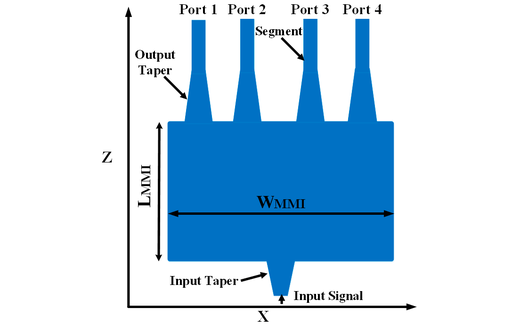
\includegraphics[width=21.6mm]{in_component.png}};
\node[tlabel] at (2.50, 2.50) {component\\[-2pt]image};
\node[thumb] (in2) at (1.28, 0.75) {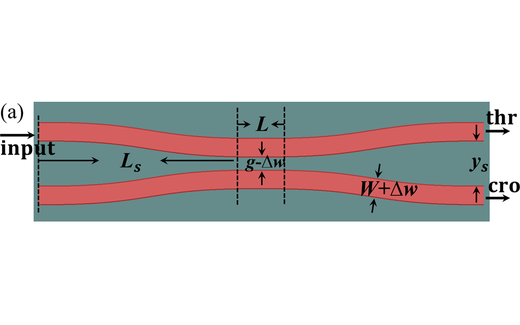
\includegraphics[width=21.6mm]{in_paper.png}};
\node[tlabel] at (2.50, 0.75) {paper\\[-2pt]figure};
\node[thumb] (in3) at (1.28,-1.00) {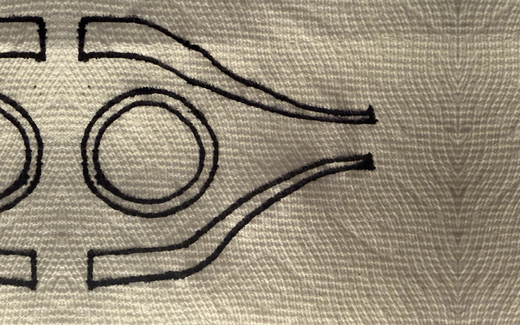
\includegraphics[width=21.6mm]{in_drawing.png}};
\node[tlabel] at (2.50,-1.00) {freehand\\[-2pt]drawing};
% studio canvas — drawn, not a screenshot
\node[thumb, fill=black!85] (in4) at (1.28,-2.75) {\phantom{\rule{21.6mm}{13.5mm}}};
\fill[black!70] (0.42,-2.19) circle (0.030) (0.54,-2.19) circle (0.030) (0.66,-2.19) circle (0.030);
\draw[white, line width=0.9pt]
  (0.62,-2.55) .. controls (1.10,-2.48) and (1.30,-2.72) .. (1.78,-2.60);
\draw[white, line width=0.9pt] (1.16,-3.02) circle (0.16);
\draw[white, line width=0.9pt]
  (0.62,-3.28) .. controls (1.10,-3.34) and (1.44,-3.18) .. (1.90,-3.26);
\draw[white, line width=0.5pt] (1.62,-2.86) -- (1.72,-2.98) -- (1.66,-2.97) -- (1.70,-3.05);
\node[tlabel] at (2.50,-2.75) {studio\\[-2pt]canvas};

% ============================== standardize ==============================
\draw[group] (4.65,-1.95) rectangle (7.65,1.95);
\node[gtitle, anchor=north] at (6.15,1.87) {standardize};

\node[thumb] (bw) at (6.15, 0.75) {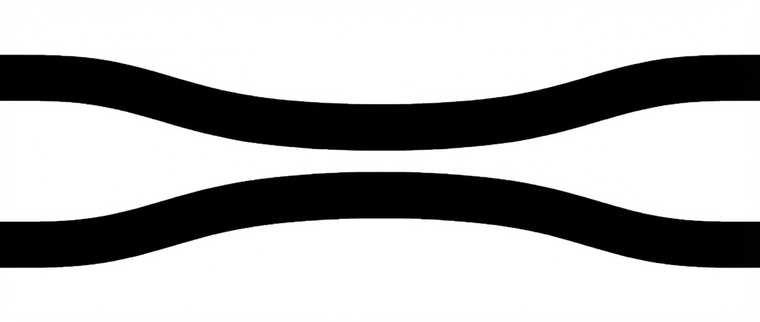
\includegraphics[width=26mm]{std_bw.png}};
\draw[{Stealth[length=1.5mm,width=1.1mm]}-{Stealth[length=1.5mm,width=1.1mm]},
      line width=0.4pt, black!60] (4.85,-0.02) -- (7.45,-0.02);
\node[font=\footnotesize, text=black!60] at (6.15,-0.24) {$18\ \mu$m $\times$ $3\ \mu$m};
\node[align=center, font=\footnotesize] at (6.15,-0.85)
  {B\&W silhouette\\[-1pt]$+$ footprint ($\mu$m)};
\node[note, align=center] at (6.15,-1.55) {deterministic ---\\[-2pt]no model in the loop};

% ================================ generate ================================
\draw[group] (8.30,-1.95) rectangle (11.90,1.95);
\node[gtitle, anchor=north] at (10.10,1.87) {generate};

\node[innerbox] (write) at (10.10, 0.85) {contained worker agent\\[-1pt]writes the program};
\node[innerbox] (verify) at (10.10,-0.90)
  {visual verifier\\[-1pt]{\footnotesize IoU at calibrated scale}};
\draw[loop] (10.70,0.42) --
  node[pos=0.5, right=2.5pt, font=\footnotesize\itshape, text=accent] {render} (10.70,-0.46);
\draw[loop] (9.50,-0.46) --
  node[pos=0.5, left=2.5pt, font=\footnotesize\itshape, text=accent] {refine} (9.50,0.42);

% ======================== artifact: verified program ========================
\node[box, font=\small] (program) at (13.90, 0.00)
  {
\includegraphics[width=19mm]{gds_raster.png}\\[2pt]
   verified parametric\\[-1pt]program\\[-1pt]{\footnotesize named tunables $\cdot$ GDS}};
\node[note, below=2.5pt of program] {the design artifact};

% ========================= decision: optimize-to-spec =========================
\node[decision] (spec) at (16.95, 0.00) {optimize-to-spec?};
\node[note, align=center] at (16.95, 1.30)
  {the spec is text: it states\\[-2pt]\emph{what} to meet, and the\\[-2pt]agent reads it};
\node[tier] (fom) at (16.95,-1.25)
  {FOM measured\\[-1pt]on the fab stack\\[-1pt]{\scriptsize mode solver $\cdot$ small FDTD}};
\draw[loop] ($(spec.south)+(0.30,0)$) to[bend left=30] ($(fom.north)+(0.30,0)$);
\draw[loop] ($(fom.north)-(0.30,0)$) to[bend left=30]
  node[pos=0.5, left=2.5pt, font=\footnotesize\itshape, text=accent] {retune} ($(spec.south)-(0.30,0)$);
\node[note] at (16.95,-2.30) {if a spec is given};

% ========================== explorer / workbench ==========================
\draw[group] (18.85,-2.65) rectangle (24.05,2.65);
\node[gtitle, anchor=north] at (21.45,2.57) {explorer / workbench};

% instrument panel
\draw[draw=black!70, line width=0.6pt, rounded corners=1.5pt, fill=white]
  (19.05,-1.95) rectangle (23.85,2.10);

% sliders — the program's named tunables
\node[font=\footnotesize, anchor=west, text=black!70] at (19.25, 1.85) {named tunables};
\foreach \y/\lbl/\kx in {1.42/gap/20.85, 1.02/$w_1$/20.30, 0.62/$L_c$/21.10} {
  \node[font=\footnotesize, anchor=east] at (19.95,\y) {\lbl};
  \draw[black!35, line width=1.0pt, line cap=round] (20.05,\y) -- (21.35,\y);
  \fill[accent] (\kx,\y) circle (0.075);
}
% per-primitive layer assignment
\node[font=\footnotesize, anchor=west, text=black!70] at (21.60, 1.85) {layers};
\fill[accent]     (21.62,1.35) rectangle +(0.14,0.14);
\node[font=\footnotesize, anchor=west] at (21.80,1.42) {guides$\,\to\,$core};
\fill[accent!40]  (21.62,0.95) rectangle +(0.14,0.14);
\node[font=\footnotesize, anchor=west] at (21.80,1.02) {trench$\,\to\,$slab};
\fill[black!45]   (21.62,0.55) rectangle +(0.14,0.14);
\node[font=\footnotesize, anchor=west] at (21.80,0.62) {pads$\,\to\,$metal};

\draw[black!15, line width=0.4pt] (19.25,0.30) -- (23.65,0.30);

% live mask + IoU
\node[thumb] at (20.05,-0.35) {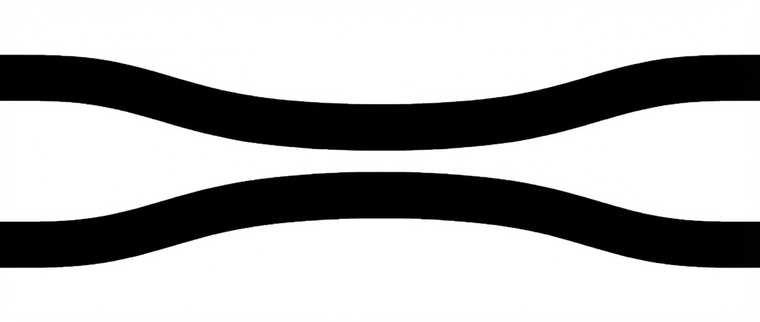
\includegraphics[width=15mm]{std_bw.png}};
\node[font=\footnotesize, anchor=center] at (20.05,-0.95)
  {live IoU \textbf{\textcolor{accent}{0.983}}};
% multi-stack view
\node[font=\footnotesize, anchor=west, text=black!70] at (21.45, 0.05) {stacks};
\node[tier, font=\scriptsize, inner sep=2.5pt, draw=accent, fill=accent!10] at (21.72,-0.40) {SOI};
\node[tier, font=\scriptsize, inner sep=2.5pt] at (22.38,-0.40) {SiN};
\node[tier, font=\scriptsize, inner sep=2.5pt] at (23.12,-0.40) {TFLN};
% talk to the agent
\draw[draw=black!50, line width=0.5pt, rounded corners=2pt, fill=black!4]
  (19.25,-1.75) rectangle (23.65,-1.30);
\node[font=\footnotesize\itshape, text=black!55, anchor=west] at (19.40,-1.52)
  {talk to the agent \ldots};
\fill[accent] (23.33,-1.62) -- (23.33,-1.42) -- (23.51,-1.52) -- cycle;

\node[note] at (21.45,-2.32) {every named tunable is a live knob};

% ================================ simulate ================================
\draw[group] (24.70,-1.95) rectangle (29.20,1.95);
\node[gtitle, anchor=north] at (26.95,1.87) {simulate};

% 2D mask glyph
\draw[draw=black!70, line width=0.5pt] (25.05,0.55) rectangle (26.15,1.30);
\draw[black, line width=1.1pt]
  (25.12,1.14) .. controls (25.42,1.14) and (25.45,0.98) .. (25.60,0.98)
                .. controls (25.75,0.98) and (25.78,1.14) .. (26.08,1.14);
\draw[black, line width=1.1pt]
  (25.12,0.70) .. controls (25.42,0.70) and (25.45,0.86) .. (25.60,0.86)
                .. controls (25.75,0.86) and (25.78,0.70) .. (26.08,0.70);
\node[font=\scriptsize, text=black!60] at (25.60,0.36) {2D mask};
% 2D -> 3D
\draw[flow, line width=0.6pt] (26.25,0.93) -- (26.90,0.93);
% 3D full-wave glyph — extruded waveguide on a substrate
\draw[draw=black!70, line width=0.5pt, fill=black!6]
  (27.05,0.58) -- (28.00,0.58) -- (28.37,0.90) -- (27.42,0.90) -- cycle;
\draw[draw=black, line width=0.6pt, fill=white]
  (27.59,0.66) -- (27.59,0.78) -- (27.94,1.08) -- (27.94,0.96) -- cycle;
\draw[draw=black, line width=0.6pt, fill=white]
  (27.45,0.78) -- (27.59,0.78) -- (27.94,1.08) -- (27.80,1.08) -- cycle;
\draw[draw=black, line width=0.6pt, fill=white] (27.45,0.66) rectangle (27.59,0.78);
\draw[accent, densely dashed, line width=0.6pt] (27.52,0.72) ellipse (0.17 and 0.13);
\node[font=\scriptsize, text=black!60] at (27.70,0.36) {3D full-wave};

\node[tier, minimum width=40mm] at (26.95,-0.55) {tier 0: mode solver \ (free)};
\node[tier, minimum width=40mm] at (26.95,-1.25) {tier 1--2: FDTD \ (capped $\cdot$ gated)};

% ================================ main flow ================================
\draw[flow] (4.00,0) -- (4.65,0);
\draw[flow] (7.65,0) -- (8.30,0);
\draw[flow] (11.90,0) -- (program.west);
\draw[flow] (program.east) -- (spec.west);
\draw[flow] (spec.east) -- (18.85,0);
\draw[flow] (24.05,0) -- (24.70,0);

\end{tikzpicture}
\end{document}
